% e-puck IR field-of-view diagram (left: IR6+IR7, right: IR0+IR1)
% Importable fragment: requires \usepackage{tikz} in your preamble.
% Units: mm (shell diameter 70, FOV arc radius 55).  Sensor mounts and facings
% from Webots' E-puck.proto (Homeo: KheperaRobot.EPUCK2): 31.6 mm (IR0, IR7)
% and 33.3 mm (IR1, IR6) from the centre, inside the shell.
% Usage: % e-puck IR field-of-view diagram (left: IR6+IR7, right: IR0+IR1)
% Importable fragment: requires \usepackage{tikz} in your preamble.
% Units: mm (shell diameter 70, FOV arc radius 55).  Sensor mounts and facings
% from Webots' E-puck.proto (Homeo: KheperaRobot.EPUCK2): 31.6 mm (IR0, IR7)
% and 33.3 mm (IR1, IR6) from the centre, inside the shell.
% Usage: % e-puck IR field-of-view diagram (left: IR6+IR7, right: IR0+IR1)
% Importable fragment: requires \usepackage{tikz} in your preamble.
% Units: mm (shell diameter 70, FOV arc radius 55).  Sensor mounts and facings
% from Webots' E-puck.proto (Homeo: KheperaRobot.EPUCK2): 31.6 mm (IR0, IR7)
% and 33.3 mm (IR1, IR6) from the centre, inside the shell.
% Usage: % e-puck IR field-of-view diagram (left: IR6+IR7, right: IR0+IR1)
% Importable fragment: requires \usepackage{tikz} in your preamble.
% Units: mm (shell diameter 70, FOV arc radius 55).  Sensor mounts and facings
% from Webots' E-puck.proto (Homeo: KheperaRobot.EPUCK2): 31.6 mm (IR0, IR7)
% and 33.3 mm (IR1, IR6) from the centre, inside the shell.
% Usage: \input{Epuck-field-of-view-combined-fragment.tex} inside a figure
% environment, or copy the tikzpicture below directly into your document.
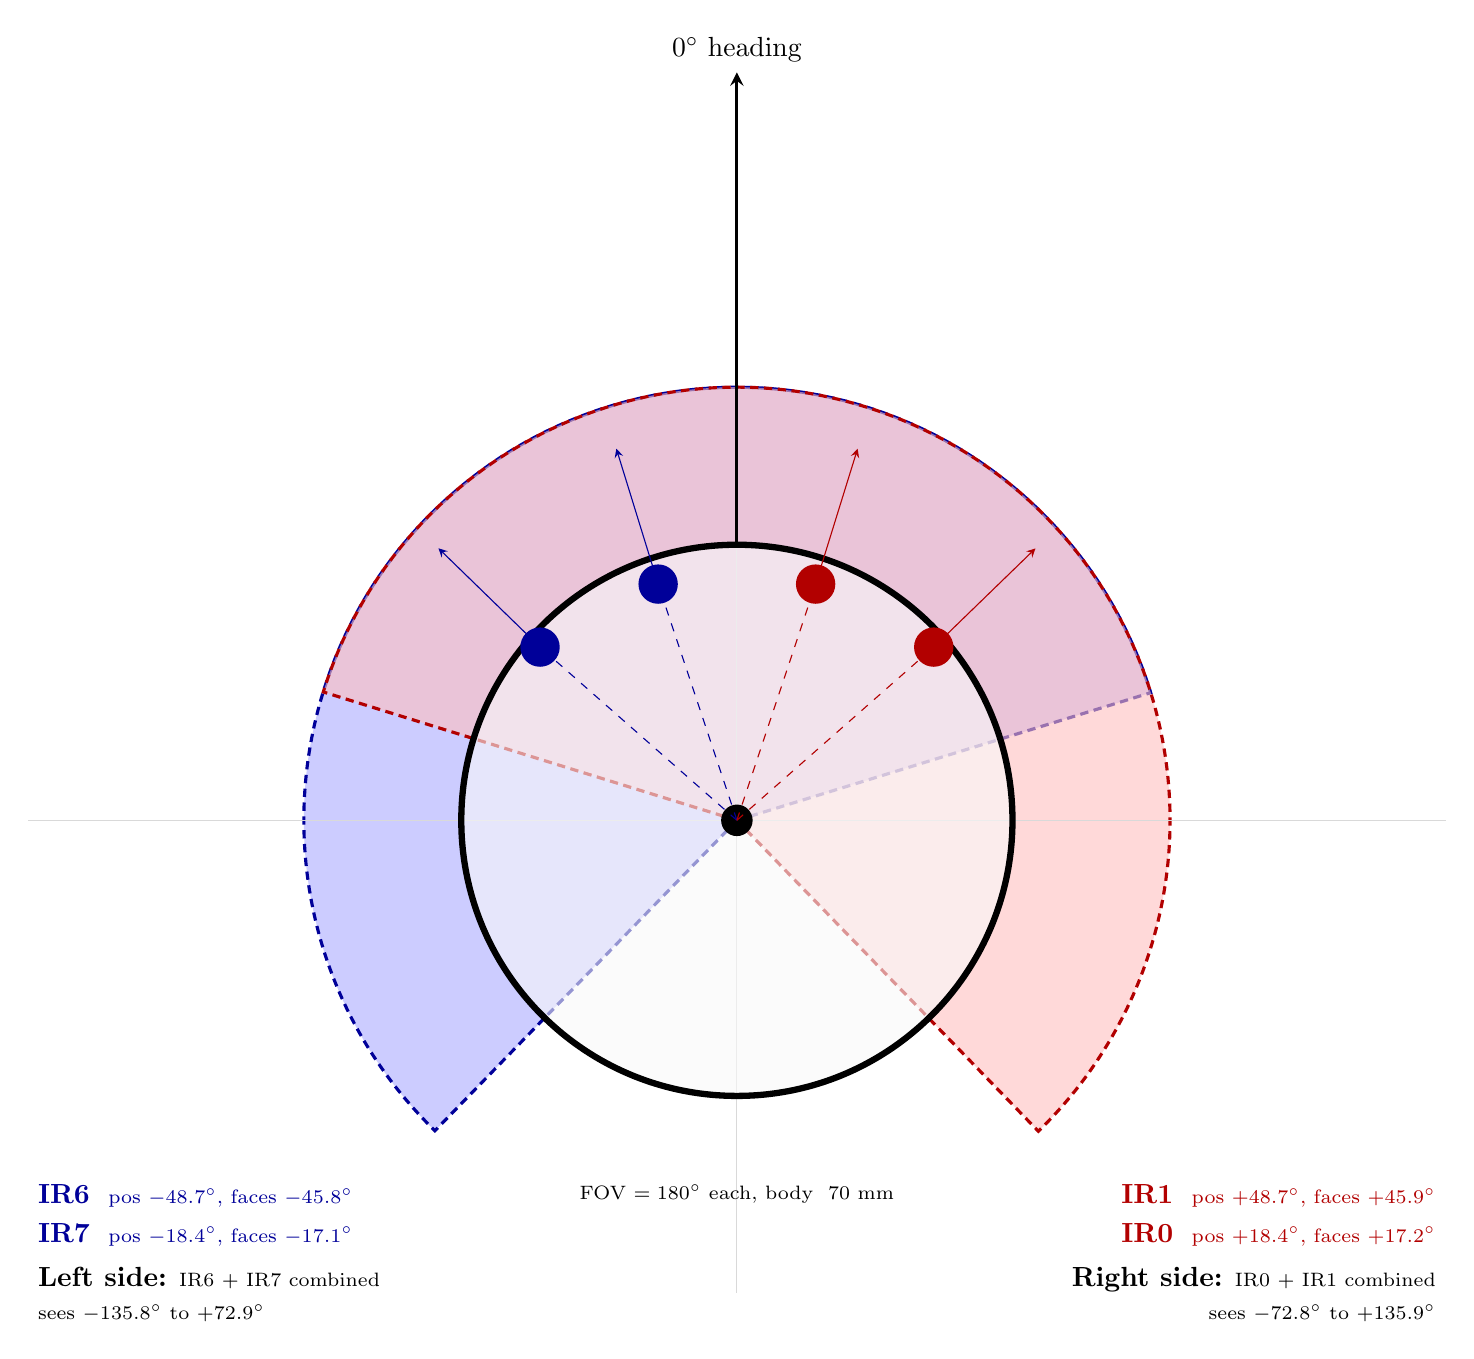
\begin{tikzpicture}[>=stealth, x=1mm, y=1mm]

  % ---- each eye's coverage seen from afar: the directions in which one of its
  % sensors has the light within its 180 degrees (near the robot the sensors'
  % offsets shift these edges) ----
  % Left (IR6 + IR7): heading -135.8 deg to +72.9 deg (std angles 225.79 -> 17.14)
  \filldraw[fill=blue!25, draw=blue!60!black, dash pattern=on 3pt off 2pt, line width=0.4mm, fill opacity=0.8]
    (0,0) -- (225.79:55)
    arc[start angle=225.79, end angle=17.14, radius=55] -- cycle;

  % Right (IR0 + IR1): heading -72.8 deg to +135.9 deg (std angles 162.76 -> -45.88)
  \filldraw[fill=red!25, draw=red!70!black, dash pattern=on 3pt off 2pt, line width=0.4mm, fill opacity=0.6]
    (0,0) -- (162.76:55)
    arc[start angle=162.76, end angle=-45.88, radius=55] -- cycle;

  % ---- grid / axes ----
  \draw[gray!30] (-90,0) -- (90,0);
  \draw[gray!30] (0,-60) -- (0,90);

  % ---- robot body: shell, 70 mm diameter ----
  \draw[line width=0.8mm, fill=gray!5, fill opacity=0.6] (0,0) circle (35);
  \fill (0,0) circle (2);

  % ---- heading reference (0 deg) ----
  \draw[->, line width=0.4mm] (0,35) -- (0,95)
      node[above, black] {$0^\circ$ heading};

  % ---- position rays, facing arrows, mount points ----
  \draw[blue!60!black, dashed, thin] (0,0) -- (-25.00,22.00);
  \draw[blue!60!black, dashed, thin] (0,0) -- (-10.00,30.00);
  \draw[->, blue!60!black] (-25.00,22.00) -- (-37.90,34.55);
  \draw[->, blue!60!black] (-10.00,30.00) -- (-15.31,47.20);
  \fill[blue!60!black] (-25.00,22.00) circle (2.5);
  \fill[blue!60!black] (-10.00,30.00) circle (2.5);
  \draw[red!70!black, dashed, thin] (0,0) -- (25.00,22.00);
  \draw[red!70!black, dashed, thin] (0,0) -- (10.00,30.00);
  \draw[->, red!70!black] (25.00,22.00) -- (37.92,34.53);
  \draw[->, red!70!black] (10.00,30.00) -- (15.33,47.19);
  \fill[red!70!black] (25.00,22.00) circle (2.5);
  \fill[red!70!black] (10.00,30.00) circle (2.5);

  % ---- legend: left side (below diagram) ----
  \node[align=left, anchor=north west] at (-90,-45)
    {\textcolor{blue!60!black}{\textbf{IR6}}\ \ \textcolor{blue!60!black}{\scriptsize pos $-48.7^\circ$, faces $-45.8^\circ$}\\[2pt]
     \textcolor{blue!60!black}{\textbf{IR7}}\ \ \textcolor{blue!60!black}{\scriptsize pos $-18.4^\circ$, faces $-17.1^\circ$}\\[4pt]
     \textbf{Left side:} \scriptsize IR6 + IR7 combined\\
     \scriptsize sees $-135.8^\circ$ to $+72.9^\circ$};

  % ---- legend: right side (below diagram) ----
  \node[align=right, anchor=north east] at (90,-45)
    {\textcolor{red!70!black}{\textbf{IR1}}\ \ \textcolor{red!70!black}{\scriptsize pos $+48.7^\circ$, faces $+45.9^\circ$}\\[2pt]
     \textcolor{red!70!black}{\textbf{IR0}}\ \ \textcolor{red!70!black}{\scriptsize pos $+18.4^\circ$, faces $+17.2^\circ$}\\[4pt]
     \textbf{Right side:} \scriptsize IR0 + IR1 combined\\
     \scriptsize sees $-72.8^\circ$ to $+135.9^\circ$};

  % ---- shared info ----
  \node[anchor=north, text=black] at (0,-45)
    {\scriptsize FOV $=180^\circ$ each, body $\varnothing$ 70 mm};

\end{tikzpicture}
 inside a figure
% environment, or copy the tikzpicture below directly into your document.
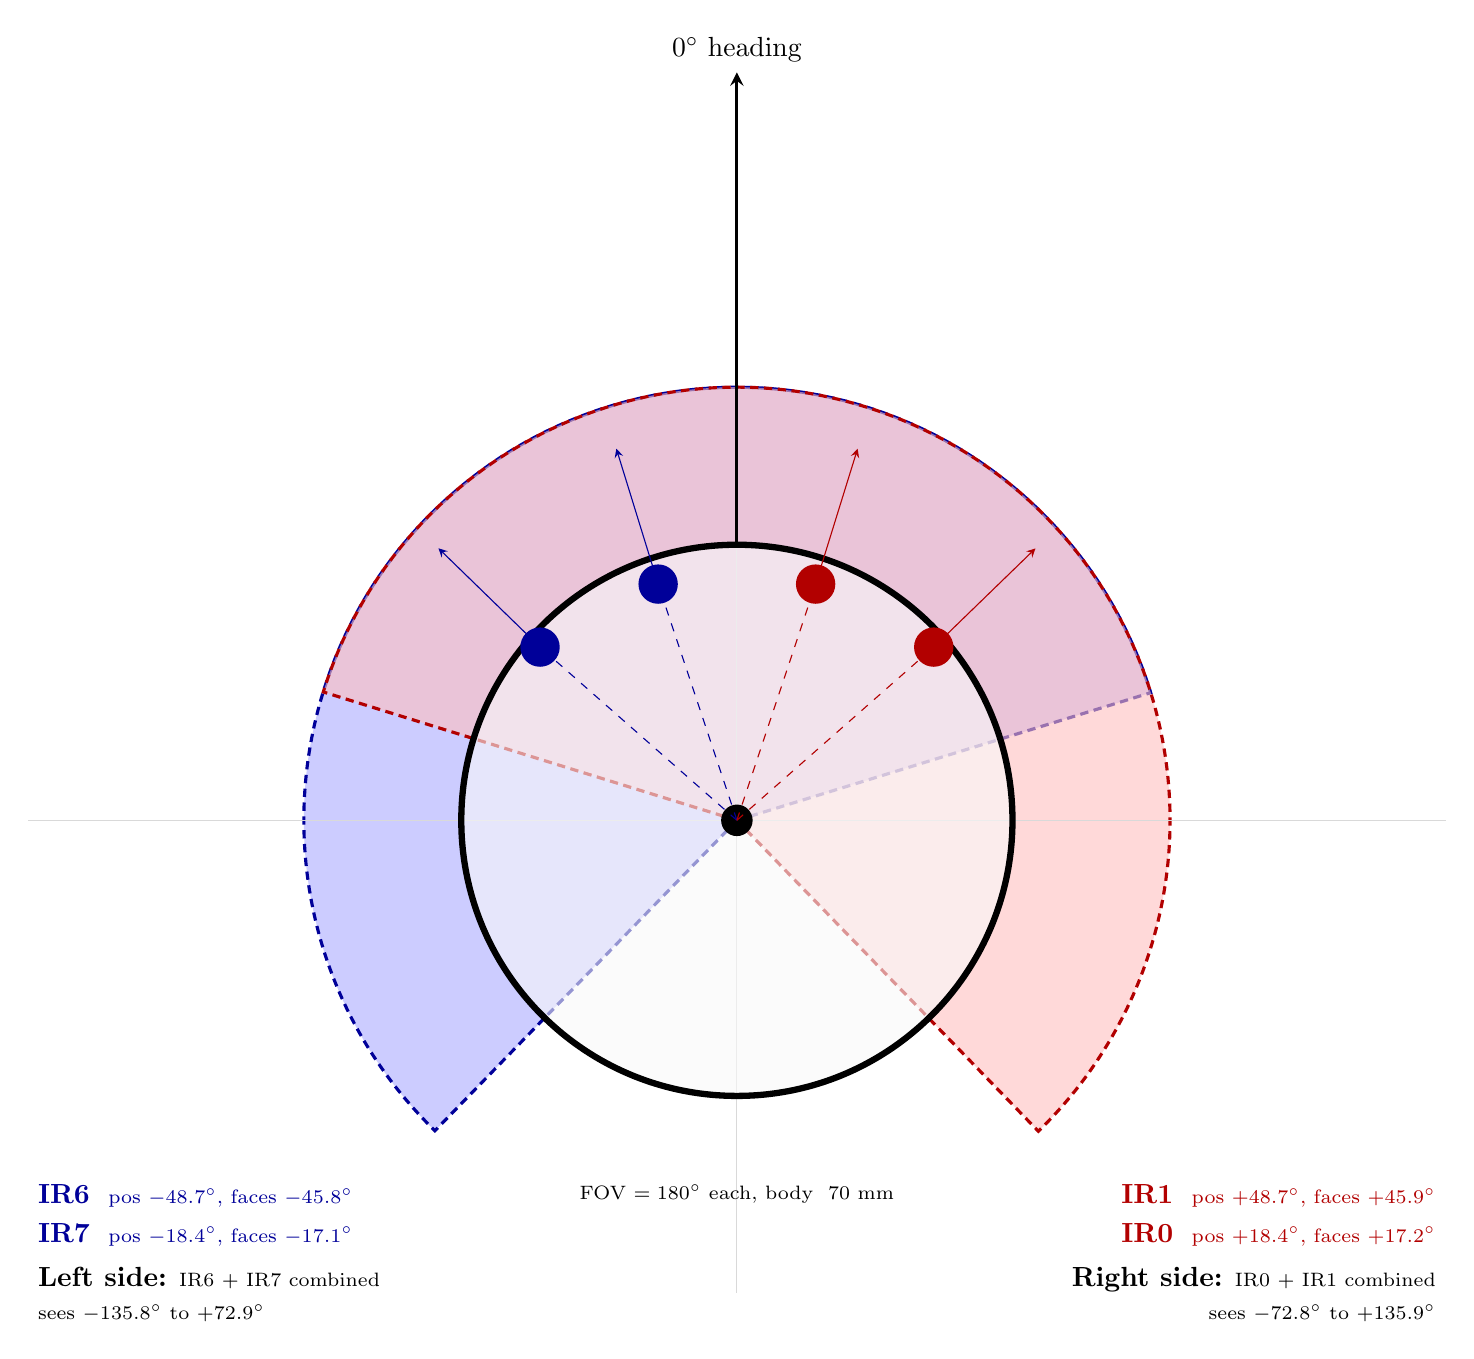
\begin{tikzpicture}[>=stealth, x=1mm, y=1mm]

  % ---- each eye's coverage seen from afar: the directions in which one of its
  % sensors has the light within its 180 degrees (near the robot the sensors'
  % offsets shift these edges) ----
  % Left (IR6 + IR7): heading -135.8 deg to +72.9 deg (std angles 225.79 -> 17.14)
  \filldraw[fill=blue!25, draw=blue!60!black, dash pattern=on 3pt off 2pt, line width=0.4mm, fill opacity=0.8]
    (0,0) -- (225.79:55)
    arc[start angle=225.79, end angle=17.14, radius=55] -- cycle;

  % Right (IR0 + IR1): heading -72.8 deg to +135.9 deg (std angles 162.76 -> -45.88)
  \filldraw[fill=red!25, draw=red!70!black, dash pattern=on 3pt off 2pt, line width=0.4mm, fill opacity=0.6]
    (0,0) -- (162.76:55)
    arc[start angle=162.76, end angle=-45.88, radius=55] -- cycle;

  % ---- grid / axes ----
  \draw[gray!30] (-90,0) -- (90,0);
  \draw[gray!30] (0,-60) -- (0,90);

  % ---- robot body: shell, 70 mm diameter ----
  \draw[line width=0.8mm, fill=gray!5, fill opacity=0.6] (0,0) circle (35);
  \fill (0,0) circle (2);

  % ---- heading reference (0 deg) ----
  \draw[->, line width=0.4mm] (0,35) -- (0,95)
      node[above, black] {$0^\circ$ heading};

  % ---- position rays, facing arrows, mount points ----
  \draw[blue!60!black, dashed, thin] (0,0) -- (-25.00,22.00);
  \draw[blue!60!black, dashed, thin] (0,0) -- (-10.00,30.00);
  \draw[->, blue!60!black] (-25.00,22.00) -- (-37.90,34.55);
  \draw[->, blue!60!black] (-10.00,30.00) -- (-15.31,47.20);
  \fill[blue!60!black] (-25.00,22.00) circle (2.5);
  \fill[blue!60!black] (-10.00,30.00) circle (2.5);
  \draw[red!70!black, dashed, thin] (0,0) -- (25.00,22.00);
  \draw[red!70!black, dashed, thin] (0,0) -- (10.00,30.00);
  \draw[->, red!70!black] (25.00,22.00) -- (37.92,34.53);
  \draw[->, red!70!black] (10.00,30.00) -- (15.33,47.19);
  \fill[red!70!black] (25.00,22.00) circle (2.5);
  \fill[red!70!black] (10.00,30.00) circle (2.5);

  % ---- legend: left side (below diagram) ----
  \node[align=left, anchor=north west] at (-90,-45)
    {\textcolor{blue!60!black}{\textbf{IR6}}\ \ \textcolor{blue!60!black}{\scriptsize pos $-48.7^\circ$, faces $-45.8^\circ$}\\[2pt]
     \textcolor{blue!60!black}{\textbf{IR7}}\ \ \textcolor{blue!60!black}{\scriptsize pos $-18.4^\circ$, faces $-17.1^\circ$}\\[4pt]
     \textbf{Left side:} \scriptsize IR6 + IR7 combined\\
     \scriptsize sees $-135.8^\circ$ to $+72.9^\circ$};

  % ---- legend: right side (below diagram) ----
  \node[align=right, anchor=north east] at (90,-45)
    {\textcolor{red!70!black}{\textbf{IR1}}\ \ \textcolor{red!70!black}{\scriptsize pos $+48.7^\circ$, faces $+45.9^\circ$}\\[2pt]
     \textcolor{red!70!black}{\textbf{IR0}}\ \ \textcolor{red!70!black}{\scriptsize pos $+18.4^\circ$, faces $+17.2^\circ$}\\[4pt]
     \textbf{Right side:} \scriptsize IR0 + IR1 combined\\
     \scriptsize sees $-72.8^\circ$ to $+135.9^\circ$};

  % ---- shared info ----
  \node[anchor=north, text=black] at (0,-45)
    {\scriptsize FOV $=180^\circ$ each, body $\varnothing$ 70 mm};

\end{tikzpicture}
 inside a figure
% environment, or copy the tikzpicture below directly into your document.
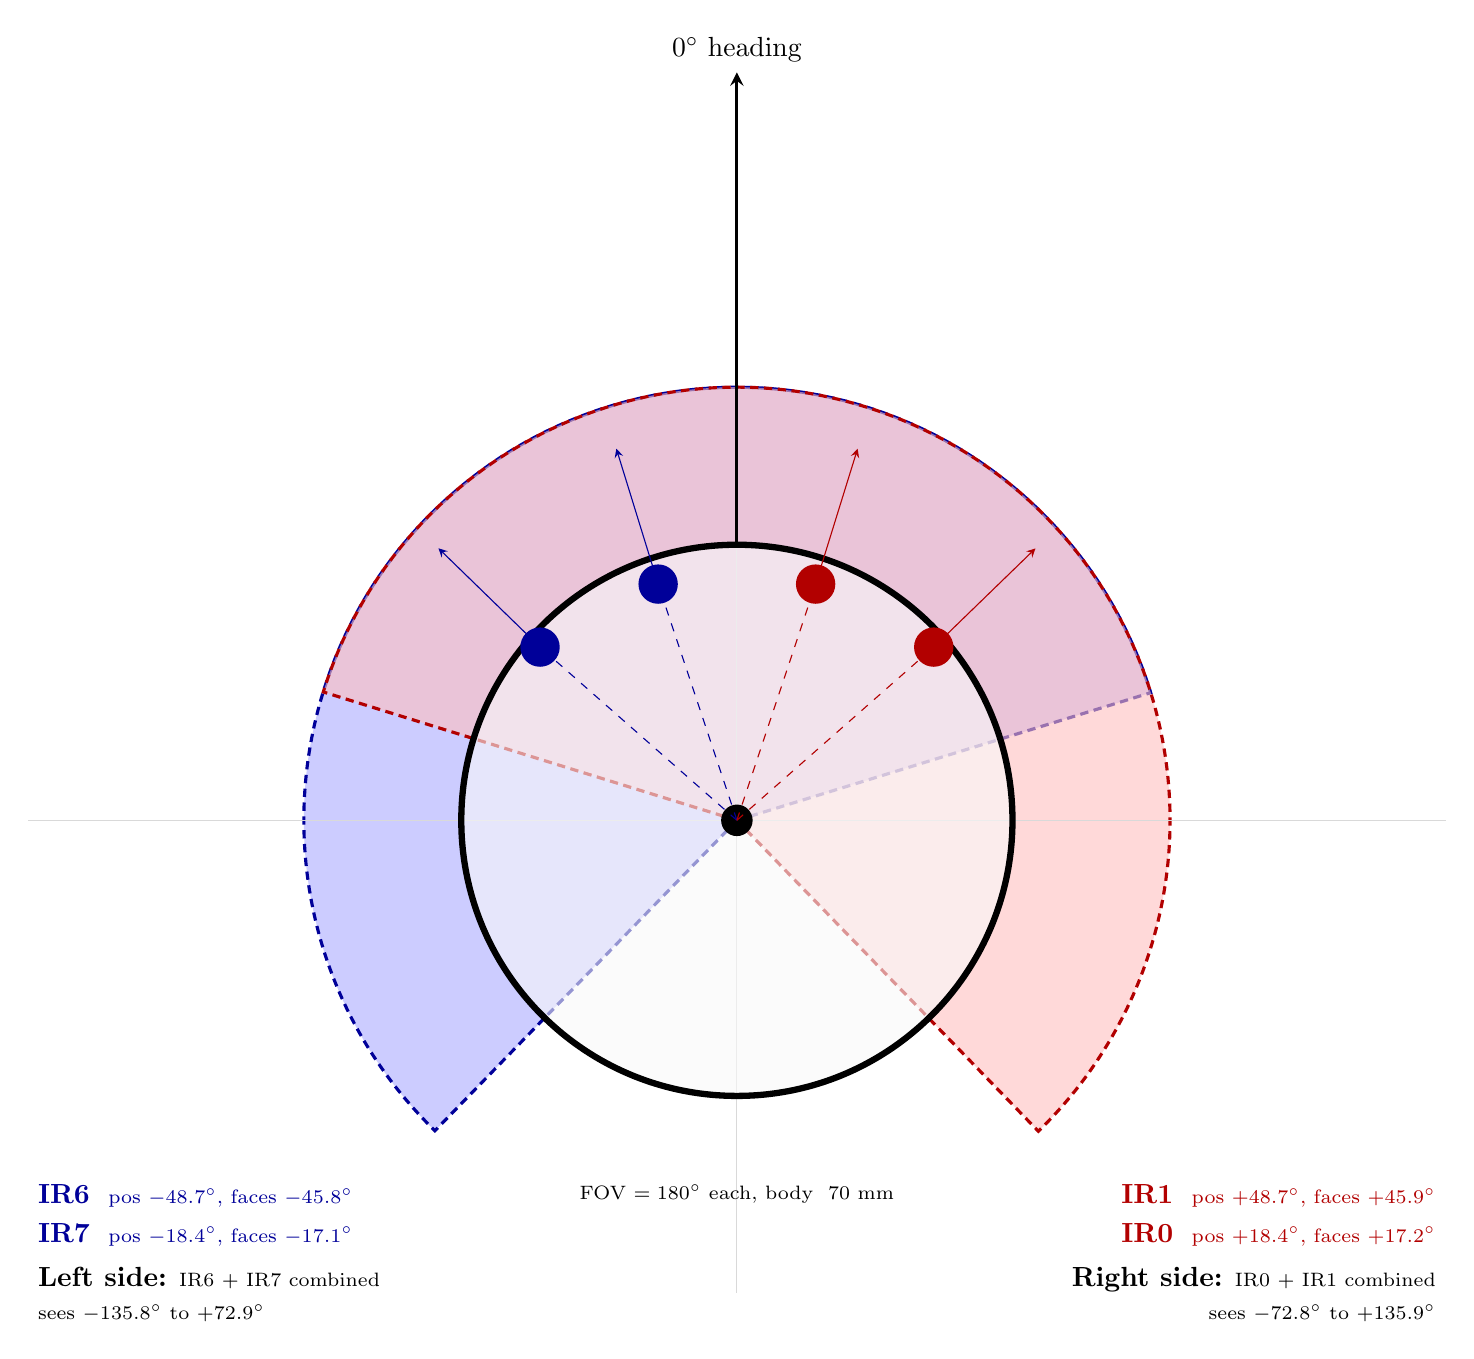
\begin{tikzpicture}[>=stealth, x=1mm, y=1mm]

  % ---- each eye's coverage seen from afar: the directions in which one of its
  % sensors has the light within its 180 degrees (near the robot the sensors'
  % offsets shift these edges) ----
  % Left (IR6 + IR7): heading -135.8 deg to +72.9 deg (std angles 225.79 -> 17.14)
  \filldraw[fill=blue!25, draw=blue!60!black, dash pattern=on 3pt off 2pt, line width=0.4mm, fill opacity=0.8]
    (0,0) -- (225.79:55)
    arc[start angle=225.79, end angle=17.14, radius=55] -- cycle;

  % Right (IR0 + IR1): heading -72.8 deg to +135.9 deg (std angles 162.76 -> -45.88)
  \filldraw[fill=red!25, draw=red!70!black, dash pattern=on 3pt off 2pt, line width=0.4mm, fill opacity=0.6]
    (0,0) -- (162.76:55)
    arc[start angle=162.76, end angle=-45.88, radius=55] -- cycle;

  % ---- grid / axes ----
  \draw[gray!30] (-90,0) -- (90,0);
  \draw[gray!30] (0,-60) -- (0,90);

  % ---- robot body: shell, 70 mm diameter ----
  \draw[line width=0.8mm, fill=gray!5, fill opacity=0.6] (0,0) circle (35);
  \fill (0,0) circle (2);

  % ---- heading reference (0 deg) ----
  \draw[->, line width=0.4mm] (0,35) -- (0,95)
      node[above, black] {$0^\circ$ heading};

  % ---- position rays, facing arrows, mount points ----
  \draw[blue!60!black, dashed, thin] (0,0) -- (-25.00,22.00);
  \draw[blue!60!black, dashed, thin] (0,0) -- (-10.00,30.00);
  \draw[->, blue!60!black] (-25.00,22.00) -- (-37.90,34.55);
  \draw[->, blue!60!black] (-10.00,30.00) -- (-15.31,47.20);
  \fill[blue!60!black] (-25.00,22.00) circle (2.5);
  \fill[blue!60!black] (-10.00,30.00) circle (2.5);
  \draw[red!70!black, dashed, thin] (0,0) -- (25.00,22.00);
  \draw[red!70!black, dashed, thin] (0,0) -- (10.00,30.00);
  \draw[->, red!70!black] (25.00,22.00) -- (37.92,34.53);
  \draw[->, red!70!black] (10.00,30.00) -- (15.33,47.19);
  \fill[red!70!black] (25.00,22.00) circle (2.5);
  \fill[red!70!black] (10.00,30.00) circle (2.5);

  % ---- legend: left side (below diagram) ----
  \node[align=left, anchor=north west] at (-90,-45)
    {\textcolor{blue!60!black}{\textbf{IR6}}\ \ \textcolor{blue!60!black}{\scriptsize pos $-48.7^\circ$, faces $-45.8^\circ$}\\[2pt]
     \textcolor{blue!60!black}{\textbf{IR7}}\ \ \textcolor{blue!60!black}{\scriptsize pos $-18.4^\circ$, faces $-17.1^\circ$}\\[4pt]
     \textbf{Left side:} \scriptsize IR6 + IR7 combined\\
     \scriptsize sees $-135.8^\circ$ to $+72.9^\circ$};

  % ---- legend: right side (below diagram) ----
  \node[align=right, anchor=north east] at (90,-45)
    {\textcolor{red!70!black}{\textbf{IR1}}\ \ \textcolor{red!70!black}{\scriptsize pos $+48.7^\circ$, faces $+45.9^\circ$}\\[2pt]
     \textcolor{red!70!black}{\textbf{IR0}}\ \ \textcolor{red!70!black}{\scriptsize pos $+18.4^\circ$, faces $+17.2^\circ$}\\[4pt]
     \textbf{Right side:} \scriptsize IR0 + IR1 combined\\
     \scriptsize sees $-72.8^\circ$ to $+135.9^\circ$};

  % ---- shared info ----
  \node[anchor=north, text=black] at (0,-45)
    {\scriptsize FOV $=180^\circ$ each, body $\varnothing$ 70 mm};

\end{tikzpicture}
 inside a figure
% environment, or copy the tikzpicture below directly into your document.
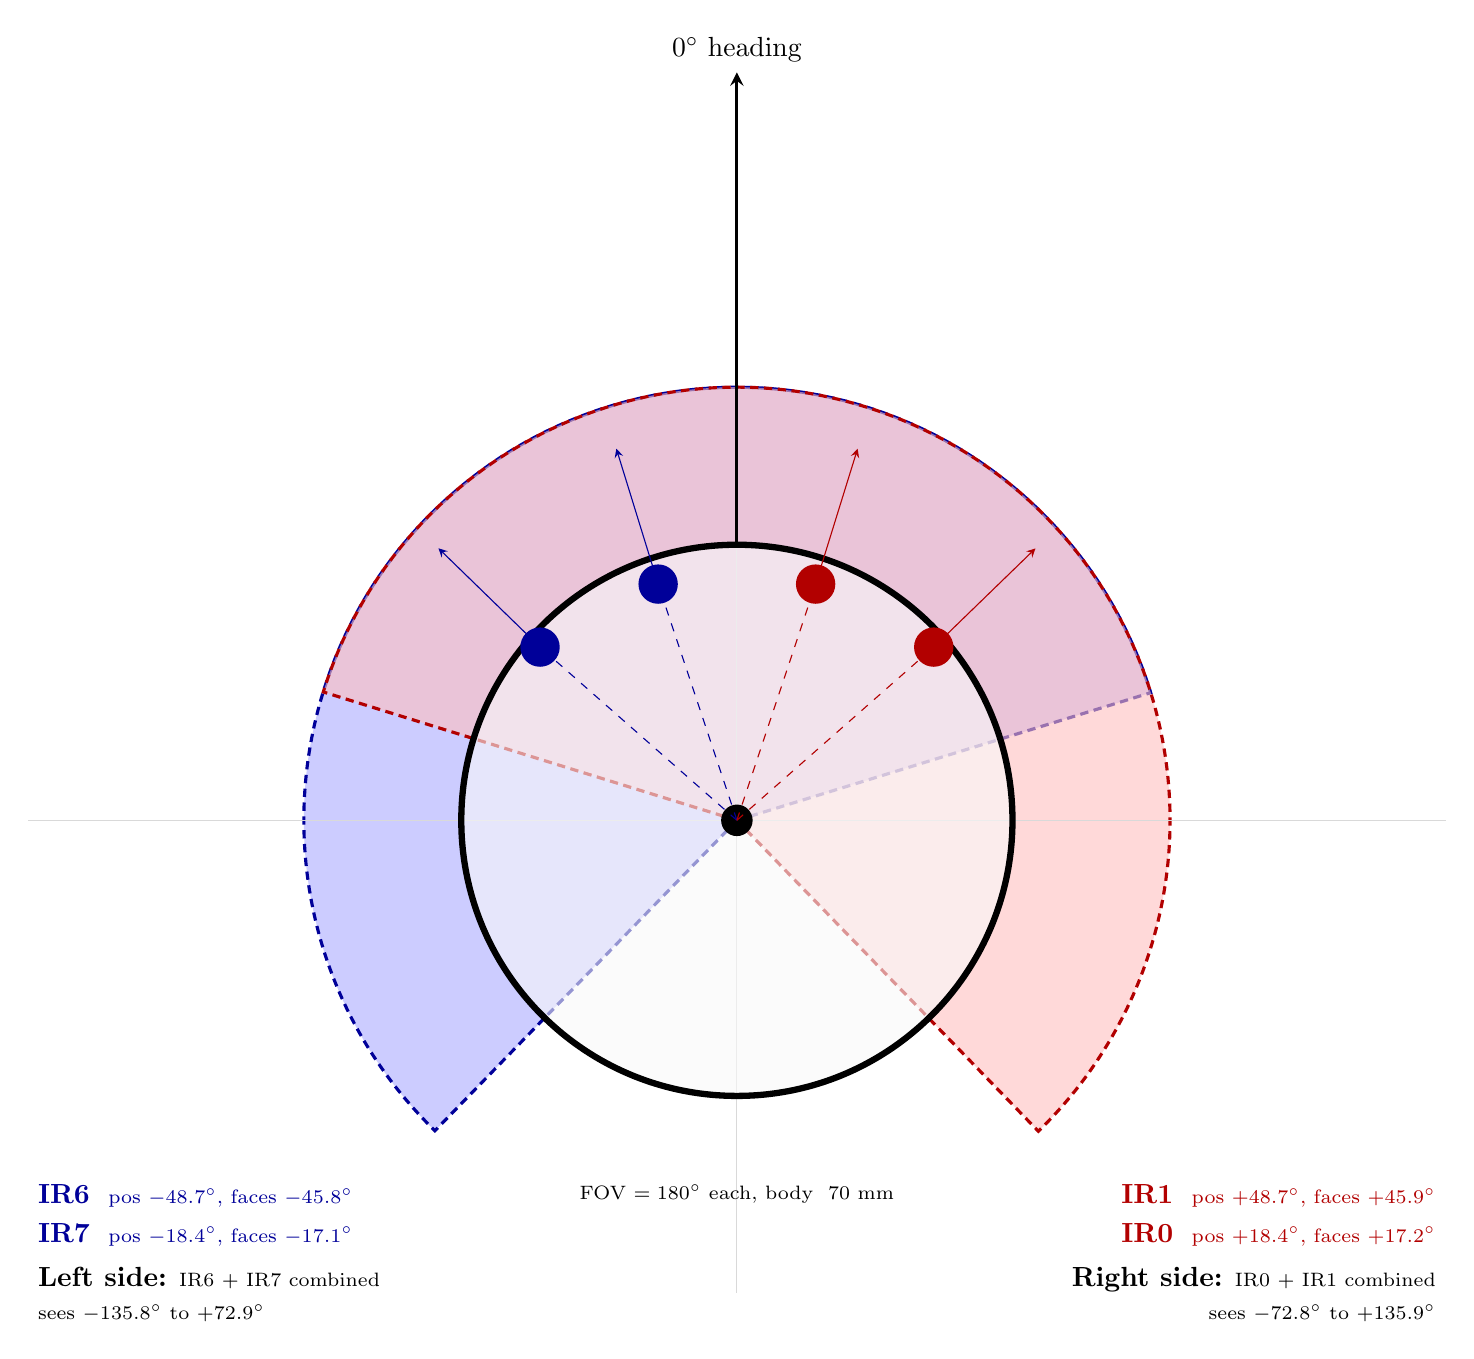
\begin{tikzpicture}[>=stealth, x=1mm, y=1mm]

  % ---- each eye's coverage seen from afar: the directions in which one of its
  % sensors has the light within its 180 degrees (near the robot the sensors'
  % offsets shift these edges) ----
  % Left (IR6 + IR7): heading -135.8 deg to +72.9 deg (std angles 225.79 -> 17.14)
  \filldraw[fill=blue!25, draw=blue!60!black, dash pattern=on 3pt off 2pt, line width=0.4mm, fill opacity=0.8]
    (0,0) -- (225.79:55)
    arc[start angle=225.79, end angle=17.14, radius=55] -- cycle;

  % Right (IR0 + IR1): heading -72.8 deg to +135.9 deg (std angles 162.76 -> -45.88)
  \filldraw[fill=red!25, draw=red!70!black, dash pattern=on 3pt off 2pt, line width=0.4mm, fill opacity=0.6]
    (0,0) -- (162.76:55)
    arc[start angle=162.76, end angle=-45.88, radius=55] -- cycle;

  % ---- grid / axes ----
  \draw[gray!30] (-90,0) -- (90,0);
  \draw[gray!30] (0,-60) -- (0,90);

  % ---- robot body: shell, 70 mm diameter ----
  \draw[line width=0.8mm, fill=gray!5, fill opacity=0.6] (0,0) circle (35);
  \fill (0,0) circle (2);

  % ---- heading reference (0 deg) ----
  \draw[->, line width=0.4mm] (0,35) -- (0,95)
      node[above, black] {$0^\circ$ heading};

  % ---- position rays, facing arrows, mount points ----
  \draw[blue!60!black, dashed, thin] (0,0) -- (-25.00,22.00);
  \draw[blue!60!black, dashed, thin] (0,0) -- (-10.00,30.00);
  \draw[->, blue!60!black] (-25.00,22.00) -- (-37.90,34.55);
  \draw[->, blue!60!black] (-10.00,30.00) -- (-15.31,47.20);
  \fill[blue!60!black] (-25.00,22.00) circle (2.5);
  \fill[blue!60!black] (-10.00,30.00) circle (2.5);
  \draw[red!70!black, dashed, thin] (0,0) -- (25.00,22.00);
  \draw[red!70!black, dashed, thin] (0,0) -- (10.00,30.00);
  \draw[->, red!70!black] (25.00,22.00) -- (37.92,34.53);
  \draw[->, red!70!black] (10.00,30.00) -- (15.33,47.19);
  \fill[red!70!black] (25.00,22.00) circle (2.5);
  \fill[red!70!black] (10.00,30.00) circle (2.5);

  % ---- legend: left side (below diagram) ----
  \node[align=left, anchor=north west] at (-90,-45)
    {\textcolor{blue!60!black}{\textbf{IR6}}\ \ \textcolor{blue!60!black}{\scriptsize pos $-48.7^\circ$, faces $-45.8^\circ$}\\[2pt]
     \textcolor{blue!60!black}{\textbf{IR7}}\ \ \textcolor{blue!60!black}{\scriptsize pos $-18.4^\circ$, faces $-17.1^\circ$}\\[4pt]
     \textbf{Left side:} \scriptsize IR6 + IR7 combined\\
     \scriptsize sees $-135.8^\circ$ to $+72.9^\circ$};

  % ---- legend: right side (below diagram) ----
  \node[align=right, anchor=north east] at (90,-45)
    {\textcolor{red!70!black}{\textbf{IR1}}\ \ \textcolor{red!70!black}{\scriptsize pos $+48.7^\circ$, faces $+45.9^\circ$}\\[2pt]
     \textcolor{red!70!black}{\textbf{IR0}}\ \ \textcolor{red!70!black}{\scriptsize pos $+18.4^\circ$, faces $+17.2^\circ$}\\[4pt]
     \textbf{Right side:} \scriptsize IR0 + IR1 combined\\
     \scriptsize sees $-72.8^\circ$ to $+135.9^\circ$};

  % ---- shared info ----
  \node[anchor=north, text=black] at (0,-45)
    {\scriptsize FOV $=180^\circ$ each, body $\varnothing$ 70 mm};

\end{tikzpicture}
